\section{SMARTHEP as a European Training Network}
\label{network}
SMARTHEP is organised as a European Training Network, funded through the 2020 EU Horizon funding call. The primary aim of the network is to train 12 ESRs, whilst building synergies between HEP and industry. The network takes a novel approach to building such synergies, structuring each ESR position (a 3 year period of doctoral study) around secondments in both HEP and industry. To achieve this, the network is formed of a series of partnerships between universities, research institutes and organisations in industry, as listed in Table~\ref{partners}.

%% Populate table
\begin{table}[h!]
    \centering
    \footnotesize
    \begin{tabular}{p{2.5cm}p{7cm}}
    \hline
    Category & Partners \\\hline
    \multirow{10}{*}{Universities} & Lund University \\
    & Sorbonne University (LPNHE \& LIP) \\
    & Technische Universit\"at Dortmund \\
    & University of Bologna \\
    & University of Geneva \\
    & University of Heidelberg \\
    & University of Helsinki \\
    & University of Manchester \\
    & Universidade Santiago de Compostela (IGFAE) \\
    & Vrije Universiteit Amsterdam \\\hline
    \multirow{3}{*}{Research institutes} & CERN \\
    & CNRS \\
    & NIKHEF  \\\hline
    \multirow{6}{*}{Industry partners} & IBM France \\
    & Lightbox \\
    & Point 6 \\
    & University of Manchester Institute for Data Science and AI \\ 
    & Verizon Connect \\
    & Ximantis\\\hline
    \end{tabular}
    \caption{The 18 organisations which form the SMARTHEP network, listed by organisation type.}
    \label{partners}       
\end{table}

The network is structured as 7 Work Packages (WPs), as laid out in Figure~\ref{network-diagram}. WP1 and WP2 define the organisation of the network; WP3 and WP4 introduce the techniques and tools of real-time analysis to the network; WP5 and WP6 use said techniques and tools to produce results for HEP and industry; WP7 makes these results available and promotes their wider use and adoption.
\begin{figure*}[h!]
    \centering
    % Use the relevant command for your figure-insertion program
    % to insert the figure file. See example above.
    % If not, use
    %\vspace*{5cm}       % Give the correct figure height in cm
    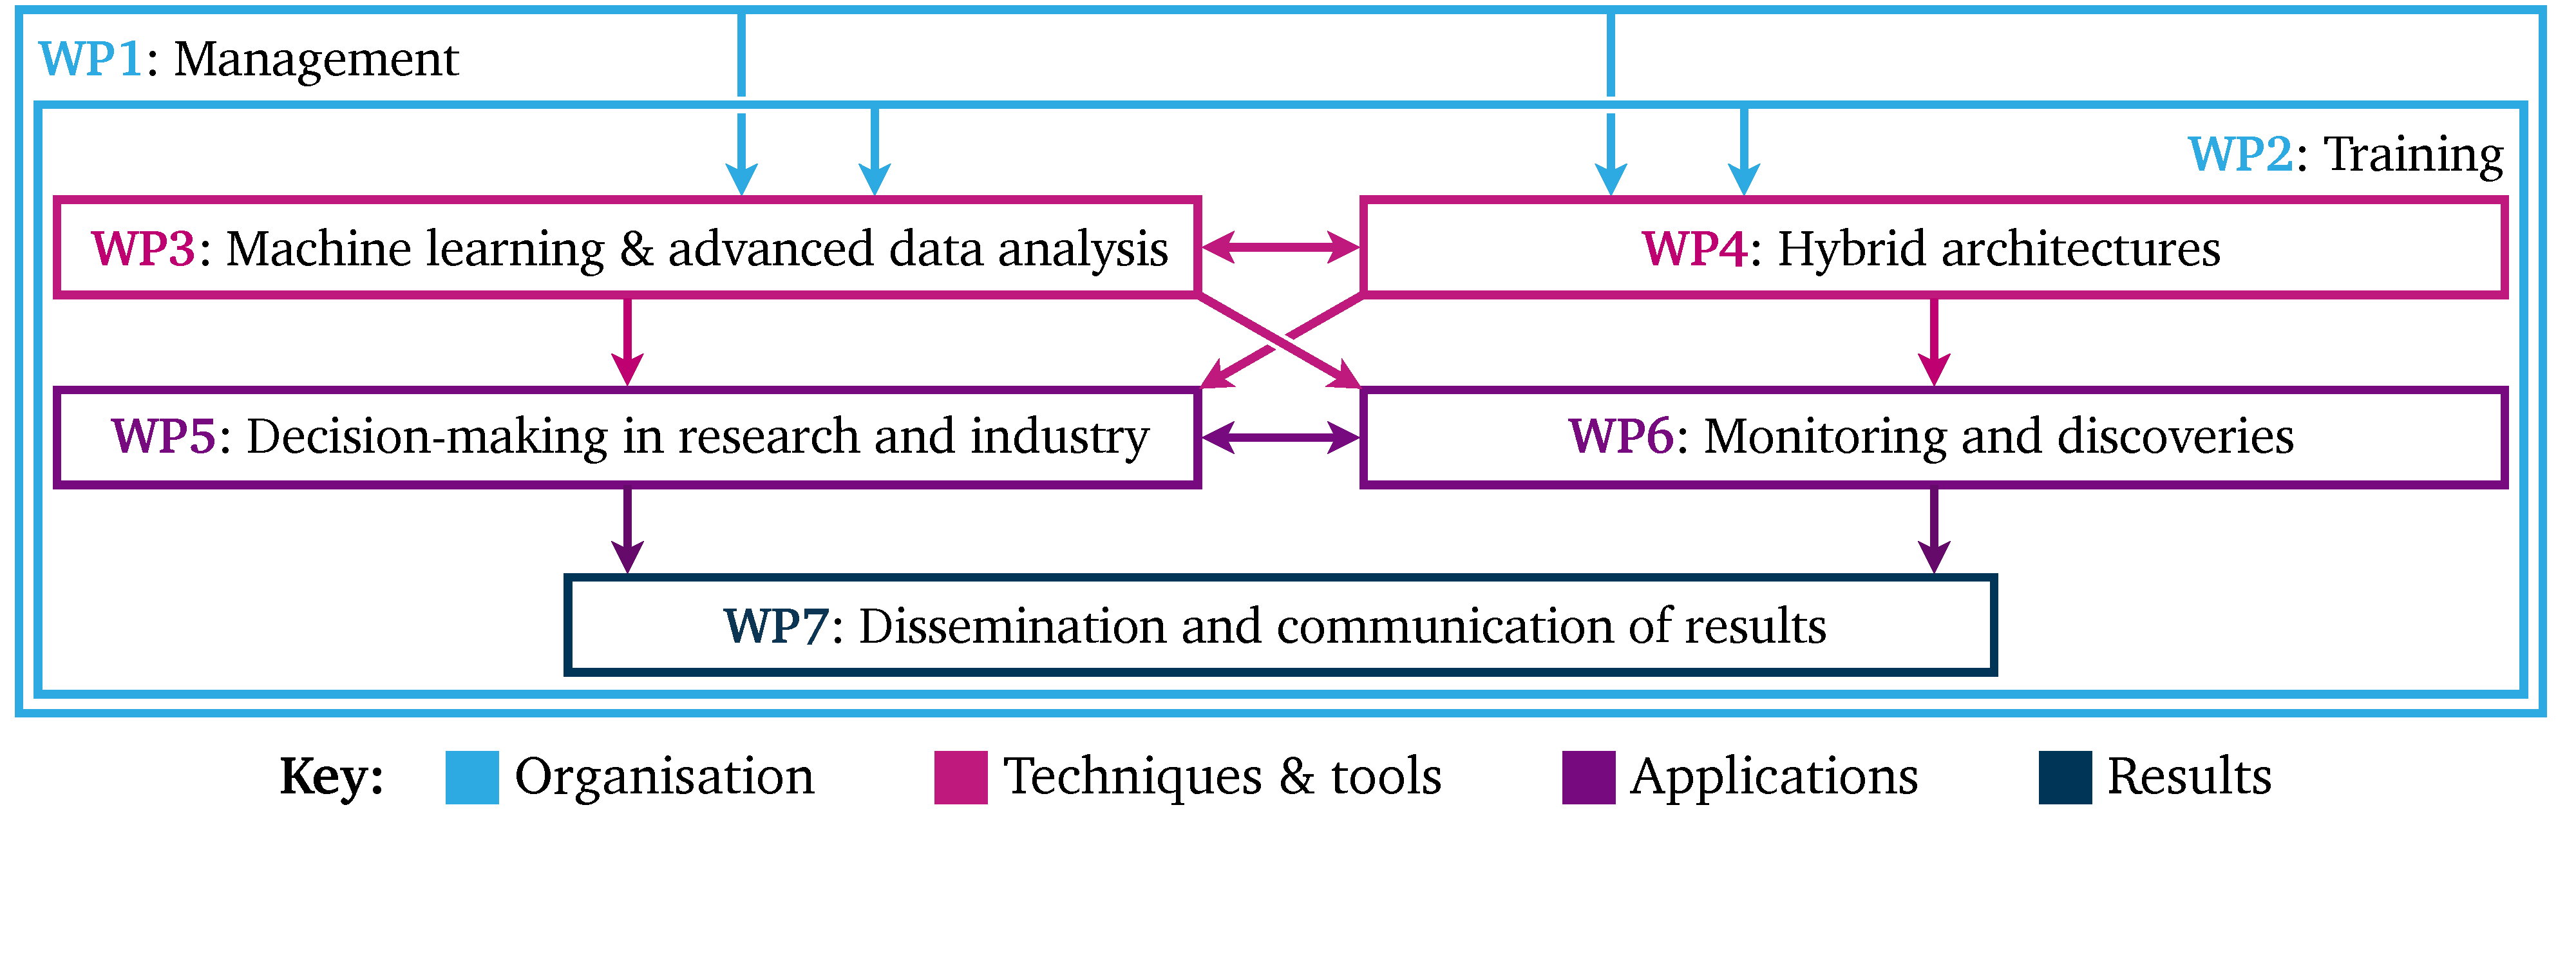
\includegraphics[width=\linewidth,clip]{/Users/jgooding/Documents/SMARTHEP/CHEP2023/CHEP2023/proceedings/figures/network-diagram.pdf}
    \caption{The structure of WPs within the SMARTHEP network. WP1, ``Management'', covers the overarching management of the network by the Project Manager, Project Coordinator, and Executive Board. WP2, ``Training'', sets out training and career development for network participants, provided by partners of the network, discussed further in Section~\ref{training}. WP3, ``Machine learning \& advanced data analysis'', develops machine learning techniques for use in RTA contexts, as discussed in Section~\ref{machine-learning}. WP4, ``Hybrid architectures'', focuses upon the deployment of non-CPU architectures for acceleration of data processing, discussed in Section~\ref{hybrid-architectures}. WP5, ``Decision-making in research and industry'', uses the work of WP3 and WP4 to develop RTA-based decision-making technologies. WP6, ``Monitoring and discoveries'', also applies WP3 and WP4 to RTA approaches in data analysis. WP7, ``Dissemination and communication of results'', publication and propagation of results from work completed by particpants. }
    \label{network-diagram}       % Give a unique label
\end{figure*}

\subsection{Partnerships with universities and research institutes}
\label{sec-2}
Within the network 
The network has a particular focus on physics at the Large Hadron Collider (LHC). Each ESR is thus affiliated to one of the four major experiments based at the LHC: ALICE, ATLAS, CMS and LHCb. The network duration coincides with Run 3 of the LHC, 2022-2025. As such, ESR projects and outcomes have a focus on delivering required work for said experiments.

\subsection{Partnerships with industry}
\label{sec-2}
A unique feature of the network is the extensive cooperation between HEP and industry across all ESR positions. RTA approaches have seen significant adoption in industry in recent years, with many organisations turning to RTA as a means to handle ``big data''.